\begin{fullwidth}
    \section{Wash Trading Profitability Analysis} \label{app:wash}

    \begin{adjustwidth}{2cm}{2cm}
        \justify
        We consider whether wash trading is profitable from the perspective of a user that both trades and stakes on dYdX Chain. We find that a wash trading strategy offers relatively low returns (<20\%) if there is sufficient value staked on the chain (we used \$200M in our example), given C=0.99 and the current v3 Trading Rewards Emissions (~\$3.2M USD per epoch). Conversely, if emissions are too high relative to total chain stake, then returns may be very high (e.g. ~75\% with \$50M staked). We find that, by introducing a minor reduction to the $C$ parameter, the dYdX protocol may effectively eliminate wash trading from the trading rewards module.
    \end{adjustwidth}
    
    \textcolor{gray}{\rule{\linewidth}{0.1mm}}
\end{fullwidth}

    We derive the conditions necessary for wash trading to be profitable as a function of the module's $C$ parameter and the emissions, $E$, it receives. We assume there is only one user wash trading on the chain, creating a conservative bound on their maximum profits. Of course, under an $N$ player game, each player competes everyone else's profits away. We base our analysis on $C=0.99$, the $C$ value discussed on a recent announcement by dYdX Trading\sidenote{Note that the $C$ parameter will be set to $0$ at Genesis.}.

    \subsection{Payoffs}

        Trading fees on Cosmos are distributed roughly \textit{pro-rata} amongst all validators every block\sidenote{Refer to \bhref{https://hub.cosmos.network/main/validators/validator-faq.html\#how-are-fees-distributed}{this} documentation for an explanation as to why.}. A user staking to a validator will therefore receive fees proportional to their staked DYDX.

        Suppose a user is staking with a validator and this validator is part of the active validator set. Further, suppose the commission rate the validator charges is $c$. The user pays $f$ in fees and receives up to $C\cdot f$ in rewards (WLOG, assume rewards are in USD). We know that the user's staking rewards will be a function of their stake and their validator’s stake relative to the chain’s total staked amount:
        
        \begin{align*}
            \text{Staking Rewards} &:= \\ &= \tfrac{\text{Validator Stake}}{\text{Chain Stake}} \cdot \tfrac{\text{User Stake}}{\text{Validator Stake}} \cdot (1 - c) \cdot f  \\ &=\tfrac{\text{User Stake}}{\text{Chain Stake}} \cdot (1 - c) \cdot f
        \end{align*}
        
        Denote the user’s stake as $s$ and the total stake as $T$, then their payoff is expressed as:
        
        \begin{equation}
            \text{Payoff} := \underbrace{\underbrace{C \cdot f}_{\text{Trading Rewards}} + \underbrace{\frac{s}{T} \cdot (1-c) \cdot f}_{\text{Staking Rewards}}}_{\text{Revenue}} - \underbrace{f}_{\text{Cost}}
        \end{equation}
        
        Notice that for a user maximizing their wash trading profits, the choice for which validator they pick is based exclusively on (1) is this validator part of the active set? and (2) what is their commission rate?
        
        For now, let’s suppose that the emissions to the trading module are infinite, then the user will want to wash trade an infinite amount if the following is true:

        \begin{equation}
            C + \frac{s}{T} \cdot (1 - c) > 1
        \end{equation}

        \subsubsection{A Strict Condition to Prevent Wash Trading}

            Let $s_{\text{max}}$ be the proportion of the chain’s stake controlled by the user with the largest staked balance, affectionately named the whale. Further, let $c_{\text{min}}$ be the lowest commission rate offered by an active validator. Then to ensure wash trading is not profitable for the whale, we must set:

            \begin{equation}
                C<1-s_{\text{max}}(1-c_{\text{min}})
            \end{equation}
            
            In doing so, we ensure that the maximum discount paid to the whale can never make wash trading profitable. Unfortunately, we cannot accurately measure $s_{\text{max}}$ since a user can split their stake among many accounts. We must then rely on estimates for how much of the chain’s stake might reasonably be controlled by a malicious agent.
            
            \begin{table}[htp]
                \centering
                \begin{tabular}{l r}
                    \toprule
                    Expected $s_{\text{max}}$ & Maximum $C$ \\
                    \midrule
                    1\% & 99.5\% \\
                    2\% & 98.1\% \\
                    5\% & 95.25\% \\
                    10\% & 90.05 \% \\
                    20\% & 81\% \\
                    \bottomrule
                \end{tabular}
                \caption{Maximum $C$ parameter to prevent wash trading given expected $s_{\text{max}}$.}
                \label{tab:C_maxes}
            \end{table}

            On Table \ref{tab:C_maxes}, we demonstrate the maximum $C$ we may set while keeping wash trading unprofitable, based on an expected $s_{\text{max}}$. 

            As it stands, the Genesis setting of $C=0.99$ allows any user with more than $\approx 1\%$ of the chain's stake to profitably wash trade under certain conditions. Of course, the larger their share of the chain's stake, the more profitable they are. If the dYdX community wants to eradicate wash trading from dYdX Chain, then it may choose to enforce a stricter condition. For example, by setting $C=0.95$, a user must command at least $\approx 5\%$ of the chain's stake to profitably wash trading. This significantly increases the initial investment required to profit from trading rewards.

    \subsection{Estimating Profits}

        To understand whether wash trading could incur meaningful losses to the dYdX protocol we derive the exact profit function for a single wash trader on dYdX Chain. This trader's profits are necessarily losses to the trading rewards program.

        By deriving optimal fees we can convince ourselves that a profitable wash trader could profit off the fees they pay, even in blocks that have relatively high volume.

        First, we return to the wash trader's payoff function and substitute $C$ for $\min{\left(\frac{E}{F_0 + f}, C\right)}$, where $F_0$ is the amount of ``organic'' fees being paid by other users. This reflects the fact that the emissions to trading rewards module, $E$, are finite, so the ``effective discount'' earned by the user can be lower than $C$:

        \begin{equation}
            \text{Payoff} := f \cdot \left(\min{\left(\frac{E}{F_0 + f}, C\right)} + s_{\text{max}} \cdot (1-c) - 1 \right)
        \end{equation}

        We can derive the optimal fees paid by first observing the shape of the payoff curve, shown in Fig \ref{fig:payoff}:

        \begin{figure}[htp]
            \centering
            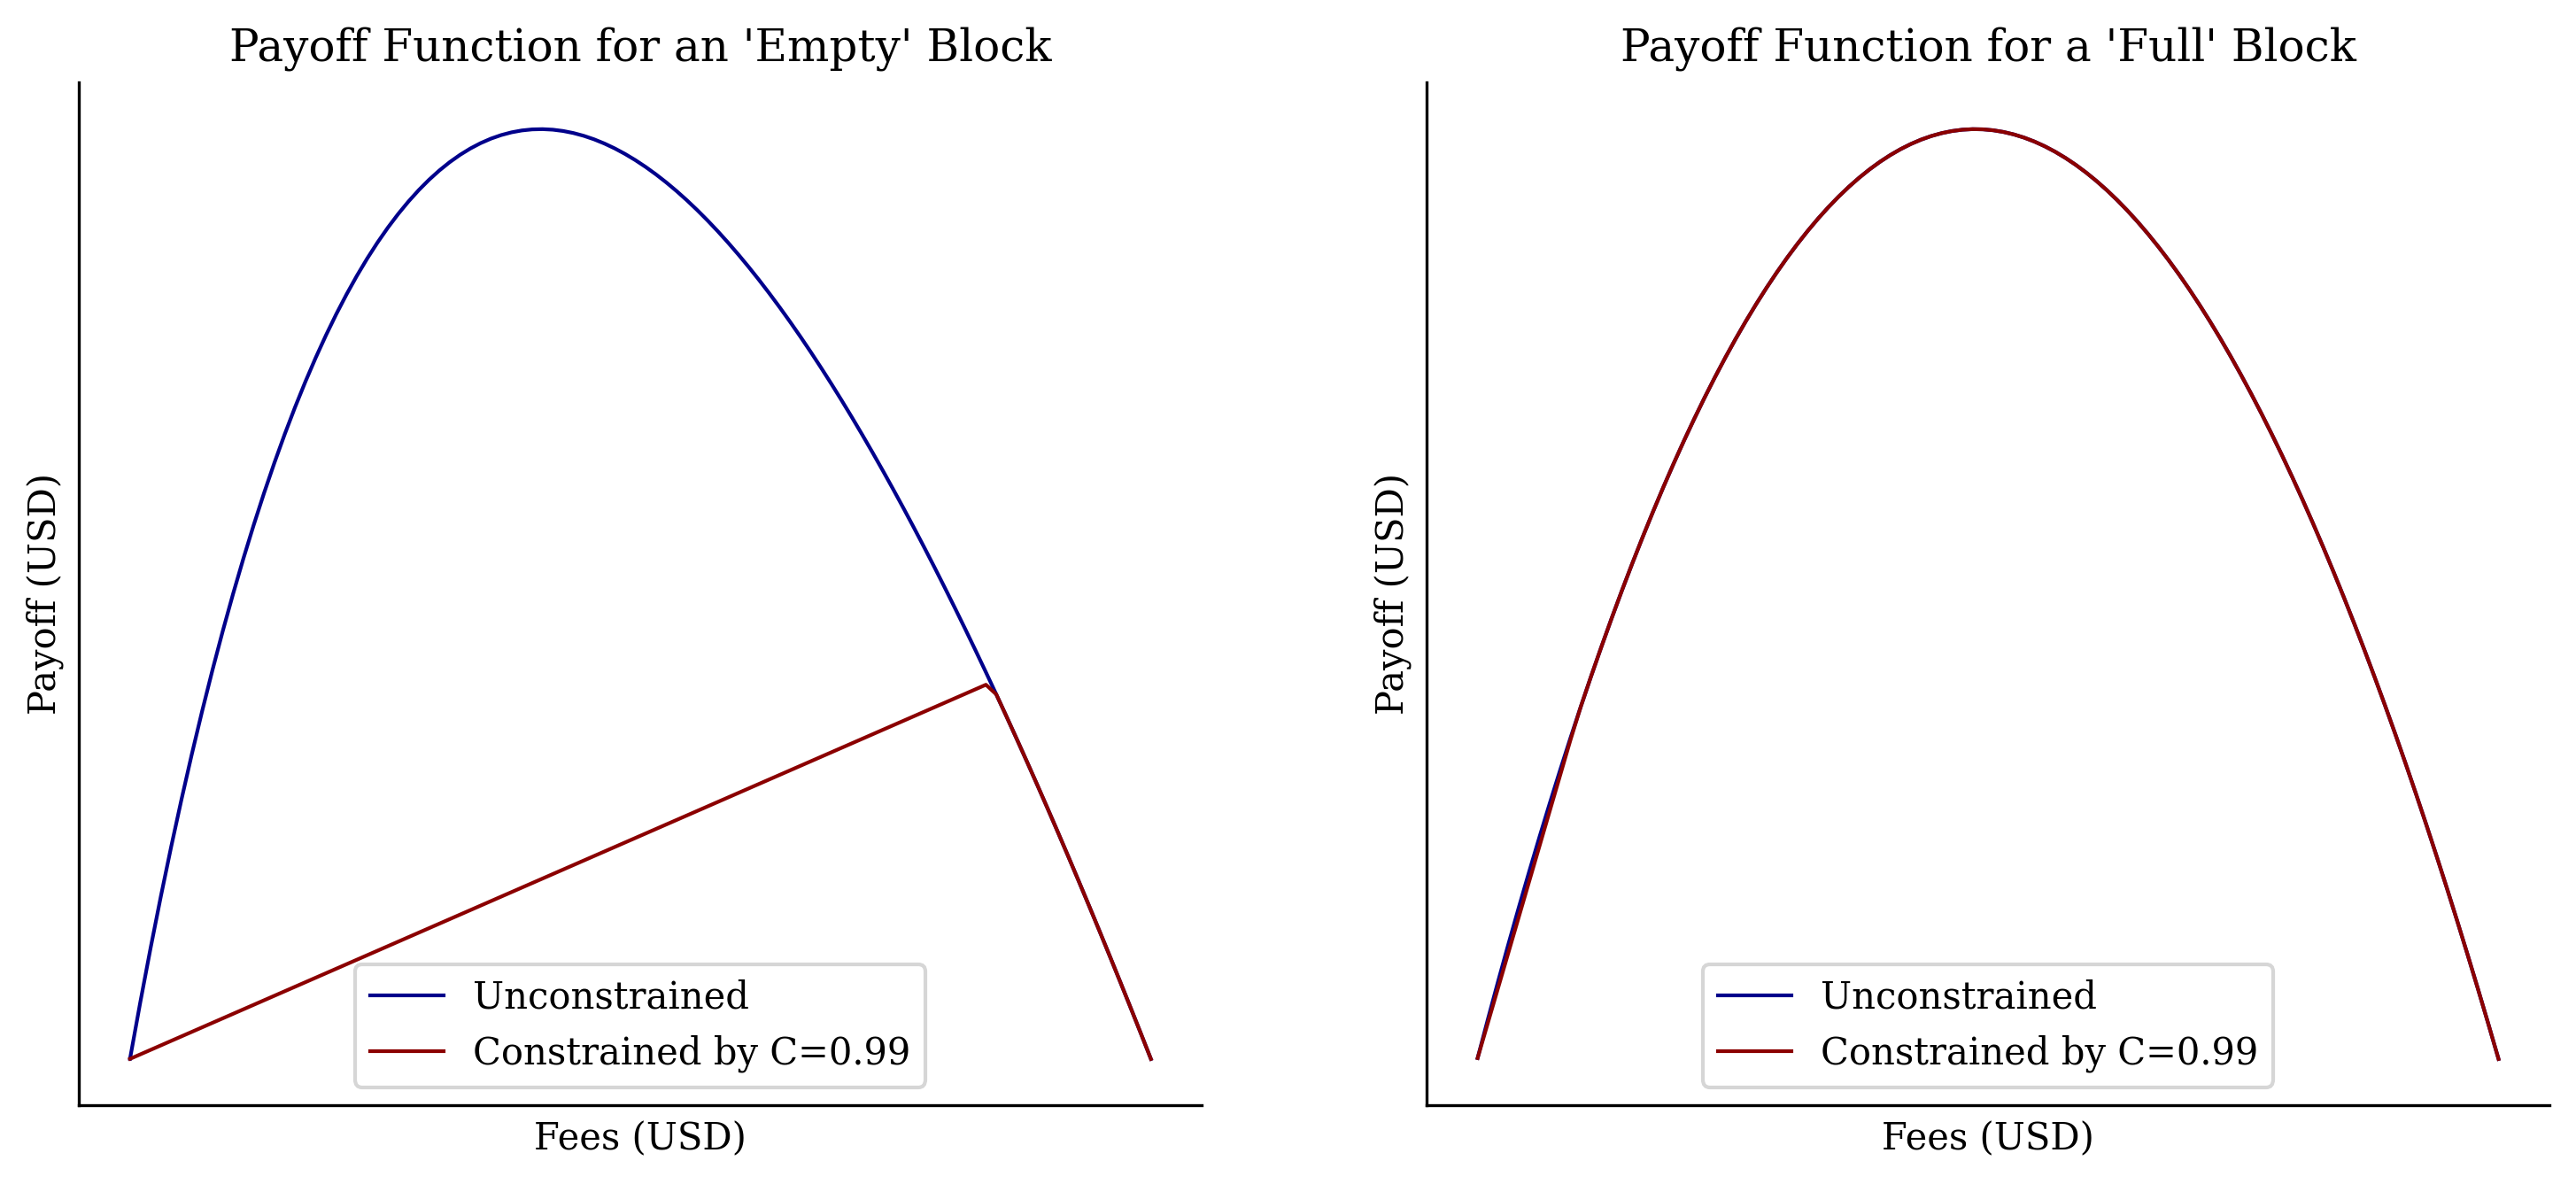
\includegraphics[width=\linewidth]{figs/payoff.png}
            \caption{User payoffs for when $F_0$ is low (an empty block) and when $F_0$ is high (a full block).}
            \label{fig:payoff}
        \end{figure}

        An ``Empty'' block is a block where $F_0 \cdot C < E$, whereas a “Full” block has $F_0 \cdot C \geq E$. The ``Constrained'' payoff involves taking the $\min{\left(\frac{E}{F_0 + f}, C\right)}$, whereas the ``Unconstrained'' problem ignores the maximum discount and simply pays $\frac{E}{F_0 + f}$ in rewards. Notice that this distinction allows us to see what the optimal strategy is for the user:

        \begin{enumerate}
            \item \textbf{Empty block:} The maximum discount constraint enforces a linear payoff until $\frac{E}{F_0 + f} < C$, at which point the payoff slopes down. Clearly, the user would pay fees until $\frac{E}{F_0 + f} = C$ so they maximize their fees at $f = \frac{E}{C} - F_0$.
            \item \textbf{Full block:} Here the effective discount will be less than the maximum discount regardless of what the user pays in fees, they therefore want to maximize
    
            \begin{equation}
                f \cdot \left(\frac{E}{F_0 + f} + s_{\text{max}} \cdot (1-c) - 1 \right),
            \end{equation}
        
            which we do with some simple calculus:
            
            \begin{align*}
                \frac{d\text{ Payoff}}{df} &= \left(\frac{E}{F_0 + f} + s_{\text{max}} \cdot (1-c) - 1 \right) - f \cdot \frac{E}{(F_0 + f)^2} \\ 
                &= \frac{E \cdot F_0}{(F_0 + f)^2} + s_{\text{max}} \cdot (1- c) - 1.
            \end{align*}
    
            Set this to 0 and solve:

            \begin{equation}
                1 - s_{\text{max}} \cdot (1-c) = \frac{E \cdot F_0}{(F_0 + f)^2},
            \end{equation}
    
            so

            \begin{equation}
                f_{\text{opt}} = \sqrt{\frac{E \cdot F_0}{1 - s_{\text{max}} \cdot (1-c)}} - F_0.
            \end{equation}
        \end{enumerate}
    

    What we find in deriving optimal fees is the following:

    \begin{equation}
        f_{\text{opt}}=\begin{cases}\max{\left(\sqrt{\frac{E\cdot F_0}{1 - s_{\text{max}}\cdot (1-c)}} - F_0,\frac{E}{C} - F_0, 0\right)} &, C > 1-s_{\text{max}} \cdot (1-c) \\ 0 &, \text{otherwise}\end{cases}
    \end{equation}
    
    With this equation, we can (1) better understand the behavior of a wash trader in different conditions (i.e. low volume and high volume blocks), and (2) estimate the losses to the protocol. This may help us determine whether wash trading is a legitimate concern.
    
    \subsubsection{Estimating Losses}

        \begin{margintable}
            \centering
            \begin{tabular}{l r}
                \toprule
                Parameter & Value \\
                \midrule
                Emissions ($E$) & 3,164,384 USD \\
                Max Discount ($C$) & 99\% \\
                Min Commission ($c$) & 5\% \\
                \bottomrule
            \end{tabular}
            \caption{Presumed parameters for Trading Rewards}
            \label{tab:tr_params}
        \end{margintable}

        Equipped with the optimal fee equation we can determine the wash trader’s maximal payoff, and therefore the community’s loss:
        
        \begin{equation}
            \text{Protocol Losses} := f_{\text{opt}} \cdot \left(\min{\left(\frac{E}{F_0 + f_{\text{opt}}}, C\right)} + s_{\text{max}}\cdot(1-c_{\text{min}}) - 1\right).
        \end{equation}

        We can also compute the wash trader's returns on invested capital (inclusive of fees):

        \begin{equation}
            \text{Returns} := \frac{f_{\text{opt}} \cdot \left(\min{\left(\frac{E}{F_0 + f_{\text{opt}}}, C\right)} + s \cdot (1-c) - 1\right) \cdot 13}{s \cdot T},
        \end{equation}
        
        where $T$ is the dollar value of the total chain stake. There are many variables here. Let’s build some intuition for protocol losses using some reasonable values. Let’s assume that the emissions are equivalent to v3 emissions, as in Table \ref{tab:tr_params}.

        From these parameters and equations, we can compute a wash trader's annualized returns using current (v3) trading rewards emissions and the Genesis $C$ parameter of 99\%. We loop through possible $s_{\text{max}} \in [0, 1]$, derive their $f_{\text{opt}}$, and then calculate the trader's returns. We graph the highest possible returns for a wash trader as a function the chain's total stake in Fig. \ref{fig:best_returns}. Notice that for reasonable total chain stakes like $\$200M$ USD, the highest possible returns for a wash trader are still pretty low given the risk and intricacy of this trade at around $20\%$.

        \begin{figure}[htp]
            \centering
            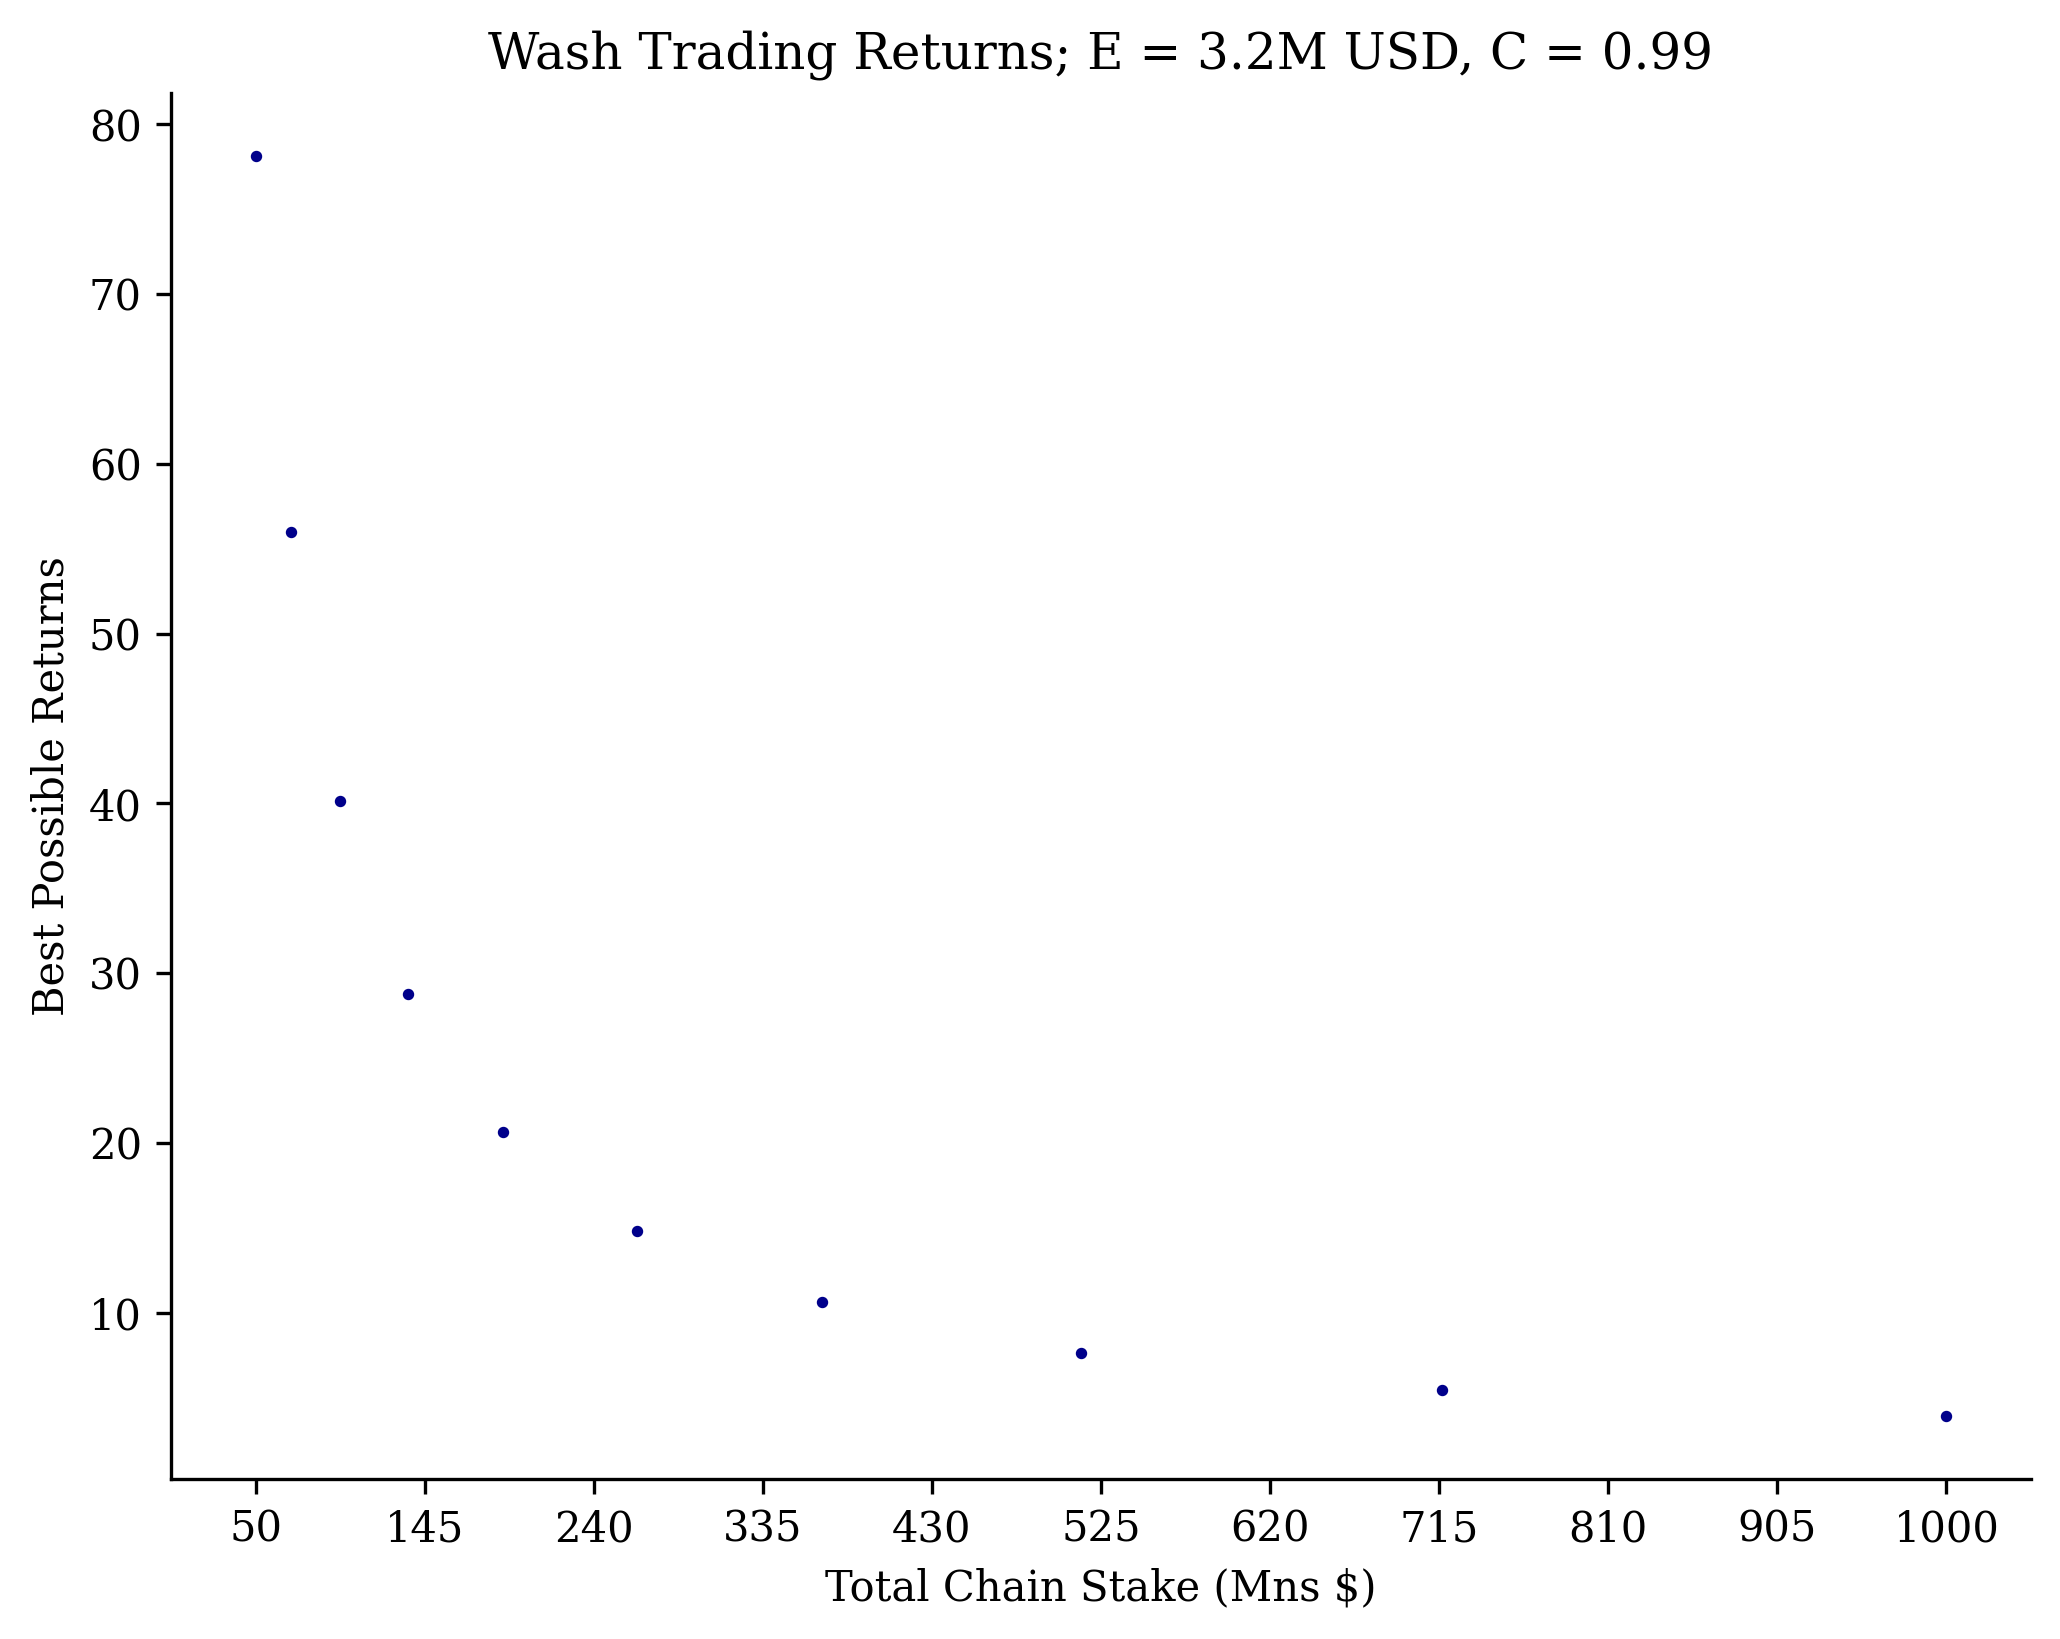
\includegraphics[width=0.7\linewidth]{figs/best_returns_3.16_0.99_0.05.png}
            \caption{Highest possible annualized returns for a wash trader assuming $\approx \$3.2M$ USD in trading rewards emitted every 28 days, or approximately $\$40M$ annualized, and $C=0.99$, as a function of total chain stake.}
            \label{fig:best_returns}
        \end{figure}

        In Fig. \ref{fig:payoff_heatmap}, we depict how the wash trader's profitability is highly sensitive to the organic flow of fees over the measurement period, as well as their share of the chain's total stake.

        \begin{figure}[htp]
            \centering
            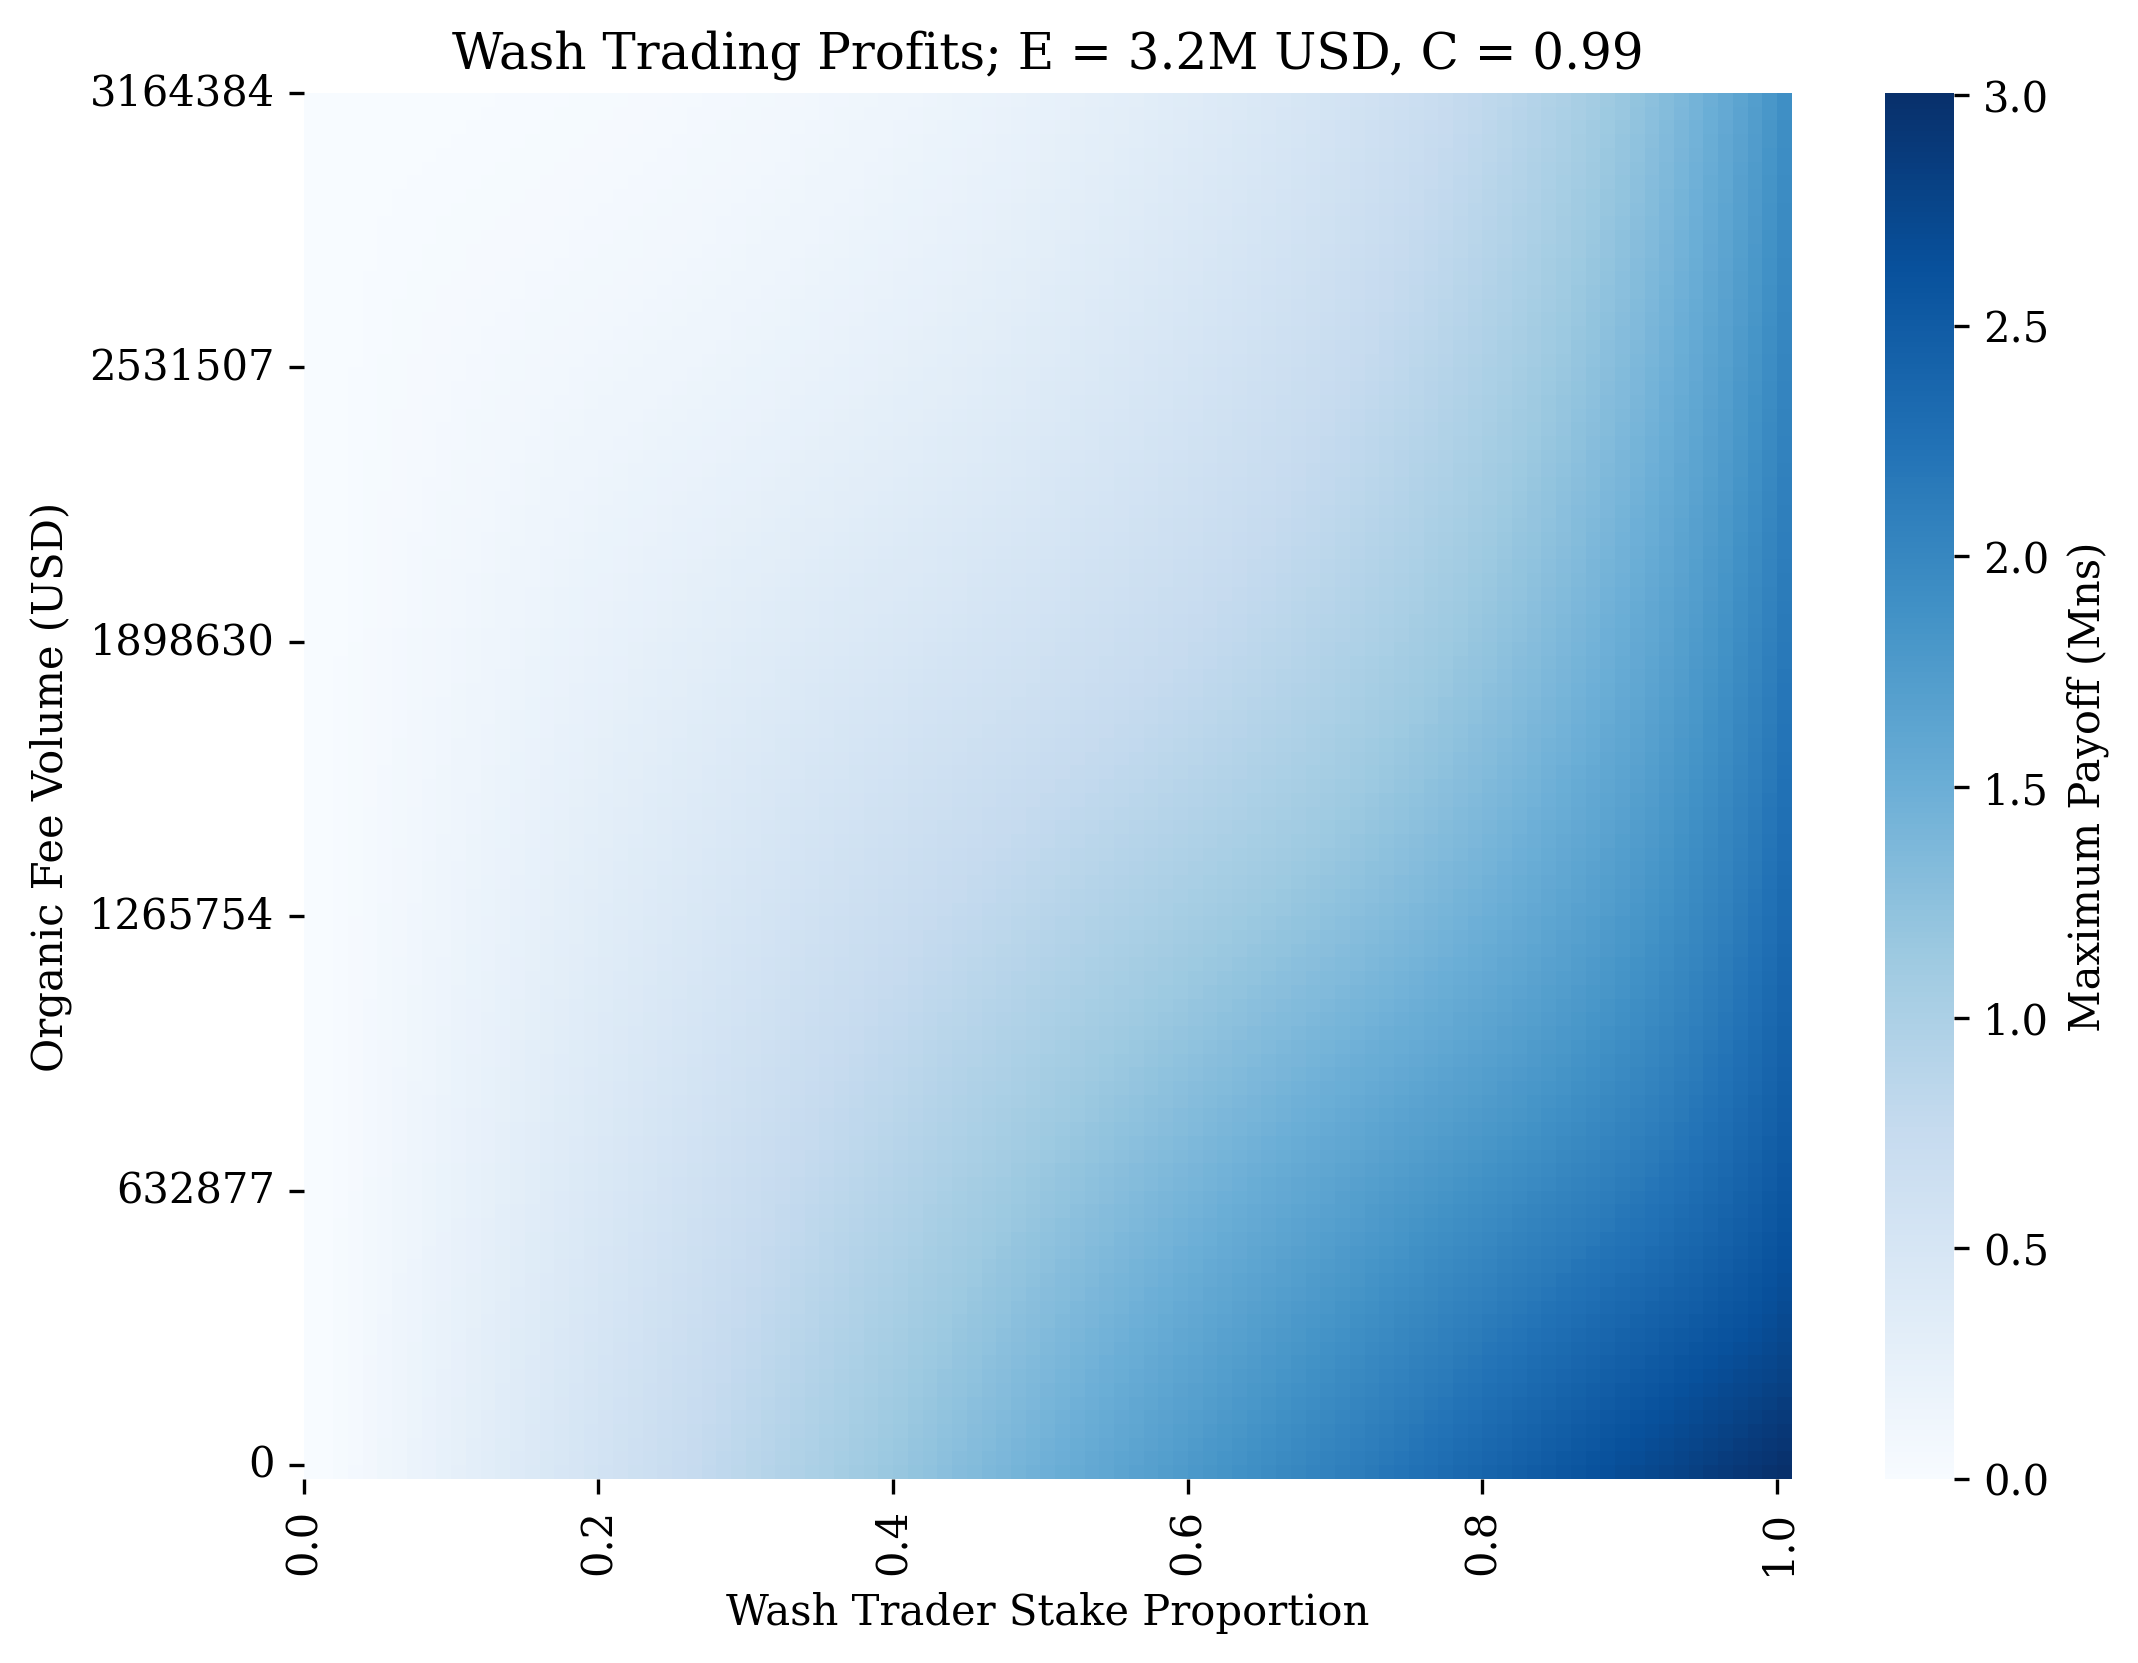
\includegraphics[width=0.7\linewidth]{figs/payoff_heatmap_3.16_0.99_0.05.png}
            \caption{Heatmap of wash trader payoff (profits) from wash trading as a function of organic fee volume and their share of total stake.}
            \label{fig:payoff_heatmap}
        \end{figure}

    \subsection{Conclusion}

        In conclusion, we can form conservative bounds on wash trader profitability, and therefore protocol losses, using the methodology outlined in this Section. Once we have an expectation on the maximum share of dYdX Chain's total stake that an adversarial agent might command, $s_{\text{max}}$, we may then set $C$ to entirely prevent them from profitably wash trading. This, of course, is a function of the total dollar value staked to the chain: if $\$1B$ USD is staked on the chain, acquiring $1\%$ of this stake is much costlier than if $\$1M$ USD is staked. 

        Once the chain launches and there is data on the dollar value of the chain's stake, as well as its general distribution, we might form reasonable expectations for $s_{\text{max}}$. Based on these expectations we may: (a) simulate the value a wash trader could siphon out of the trading rewards program, and (b) adjust $C$ to prevent them from profitably wash trading.